\chapter{Information Visualisation aspects}
\label{chapter:iv}
In this chapter, we describe all the choices and aspects of the application related to the purpose of the course which is the Information Visualisation. We also cover a part of User Experience.

%-------------------------------------------------------------------------------
%-------------------------------------------------------------------------------
\section{Target audience}
This app is provided to different financial actors, from analysts, to managers and even students. It helps the user to create a mental model bringing together what were the stocks values at a certain time and what appeared in the news around this event, which might lead to be an answer and to understand the evolution of the price.

%-------------------------------------------------------------------------------
%-------------------------------------------------------------------------------
\section{Data to visualize}
The first question to ask is what is the data we are using and what information we want to give to the user. As stated in section~\ref{sec:intro:features}, we want to give a clear picture of the different events that occured within a specific range of time (e.g. 1 year) by providing news related to the events.
For example, if the shared stock value of some company dropped on 3$^{\text{rd}}$ July 2015, the user might want to know what happened on this particular day. Thus, the app will retrieve the news that talk about the company around that day. Maybe that an article from \textit{Reuters} or \textit{Swissquote} will explain why the shared stock value lost 50 \$.

The data is numerical, quantitative and temporal (i.e. expressed with a time dimension). Defaults are set to present 1 year from the current day of stock values, 5 events occuring in this time frame, and the articles in a range of 2 months before and after the event.

In the next sections, we are describing more precisely the different information present on the app and how we decided to represent them.

%-------------------------------------------------------------------------------
\subsection{Stock values}
To represent the stock values we used a chart created with the Javascript library HighchartsJS, or more specifically, with HighstocksJS, a library using HighchartsJS. In the figure~\ref{fig:stockchart}, we see Facebook (FB) stock prices in a one year time range.
\begin{figure}
    \centering
    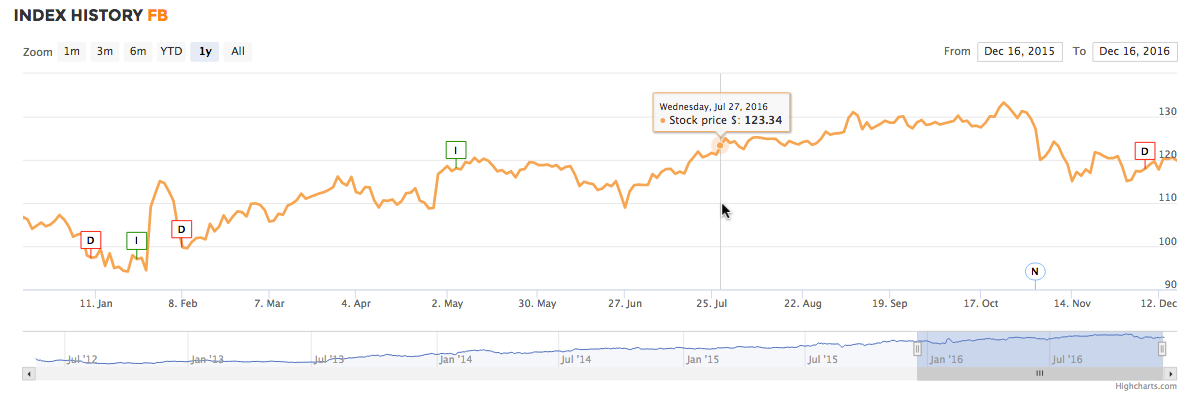
\includegraphics[max width=\textwidth]{Figures/st-chart-pointer.png}
    \caption{Example of visualisation of the Facebook (FB) stock price between the 16$^{\text{th}}$ December 2015 and 16$^{\text{th}}$ December 2016.}
    \label{fig:stockchart}
\end{figure}
There are two important visual enhancements to a simple line chart present in our chart. First, there are two visualizations of the data itself, one big of current timeframe and a second one smaller below the big one representing briefly the whole data set. And secondly, the different events were added as flags on the line to let the user visualize at first sight when the events occured. The flags are here to amplify cognition.

In addition of the visual enhancements, there is also the possibility to interact directly with the chart and zoom to a particular range, or to drag the mouse and know what we are pointing at.

As our target is financial actors, representing the line chart is what they are used to when they look at the evolution of the stock price. Thus, in order to be the least surprising to them, we decided to also use a line chart.

%-------------------------------------------------------------------------------
\subsection{Events}
Before getting at how we represented the events, let us define what an event is.
\begin{center}
    An event is understood as a ``\textit{significant decrease or increase in a short amount of time}''.
\end{center}
An event is linked to the information provided by the line chart. In order to keep this temporal dimension, we decided to represent the events on a non-scaled (i.e. the separation between the dates does not respect the actual time difference) timeline. The timeline is top-bottom, which means that the most recent event is at the top and the others follow in a reversed chronological order.

Besides the time information, we also represent the type of event. Is it an event due to a significant increase (i.e. positive event) or decrease (i.e. negative event)? To answer this question, let us consider the figure~\ref{fig:event-timeline}. An arrow facing up describes a positive event and, \textit{a contrario}, an arrow facing down describes a negative event. This information is amplified by the color. A green or red arrow is used for respectively a positive or a negative event.

The highlighted event helps the user to reminder what event is currently used to retrieve the news.

\begin{figure}
    \centering
    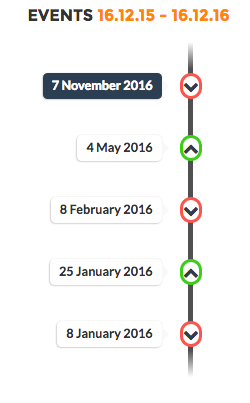
\includegraphics[scale=0.5]{Figures/st-events.png}
    \caption{Example of visualisation of the Facebook (FB) stock price events between the 16$^{\text{th}}$ December 2015 and 16$^{\text{th}}$ December 2016.}
    \label{fig:event-timeline}
\end{figure}

%-------------------------------------------------------------------------------
\subsection{News}
The news are related to an event. Each different event might output a different list of articles. Therefore, the simplest way to represent this list is using a list. The important information are the title of the article, the date when it was published and by who. All these information are visualize in the list and when the user clicks on one of the article, a description is shown, followed by the same important information. If the user wants the full article, he can click on the title and be redirected to the concerned website.

In the list, the article currently read is highlighted with a high contrast of the colors. And in addition of that, the user can also represent the article within the time by looking at the flag ``\textit{N}'' on the x-axis of the chart. This way and as the article might not have been published on the particular day of the event itself, it helps the user to visualize the time frame between the two, the article being read and the event being analyzed.

\begin{figure}
    \centering
    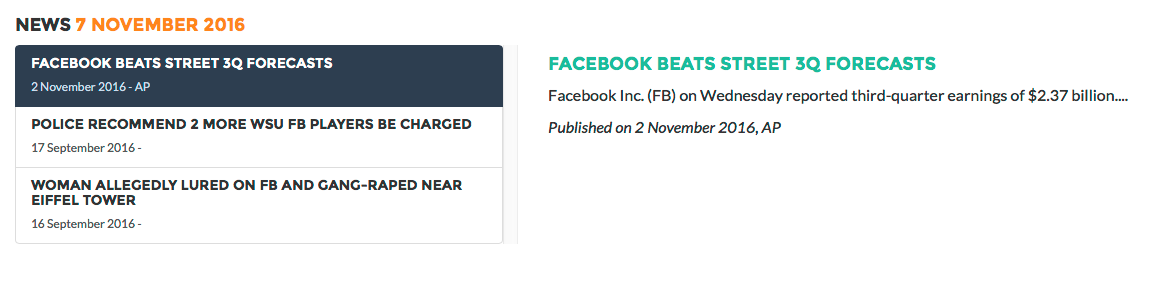
\includegraphics[max width=\textwidth]{Figures/st-news.png}
    \caption{Example of visualisation of one the event of the Facebook (FB) stock price occuring between the 16$^{\text{th}}$ December 2015 and 16$^{\text{th}}$ December 2016, precisely on the 7$^{\text{th}}$ November.}
    \label{fig:news}
\end{figure}

%-------------------------------------------------------------------------------
%-------------------------------------------------------------------------------
\section{The orange color}
As presented in the third lecture\footnote{InfoVisMSE\_03.pdf, \textit{Human perception, mental models} p.13} of the course, a different color helps the perception as a \textit{preattentive processing}, for example, to highlight information. In our case, what we are highlighting is the data that changes through the use of the application. Here is the list of the orange representations on the application.
\begin{itemize}
    \item Line in the chart
    \item Current index
    \item Events range
    \item News relevant to an event
\end{itemize}
The purpose is to catch the eye when the user does not remember the context of what he is looking at and needs a refresh. An example is presented in figure~\ref{fig:full}.

%-------------------------------------------------------------------------------
%-------------------------------------------------------------------------------
\section{User Experience}
As we can see in the figure~\ref{fig:full}, the whole application stands on a single page. It has been made this way to provide a constant overview of the information. As an analyst often has multiple screens (sometimes 6), he has to have all the information he wants fit in one screen, his eyes are already bouncing between different screens, he cannot remember in which part of the website he is at the moment. In addition of that, the first information that the user will read in a ``\textit{F}''\footnote{InfoVisMSE\_03.pdf, \textit{Human perception, mental models}, p.16} path of his eyes is the chart, followed by the list of events, and finishing by the list the news. This path is correlated with the ``overview at first sight and then go deeper'' approach.

The different interactions possible with the application are the following. The different categories are from the 6$^{\text{th}}$ lecture\footnote{InfoVisMSE\_06.pdf, \textit{Interaction}, p.8} of the course.
\begin{itemize}
    \item \textbf{Explore}: the user can change the index, drag his mouse on the chart to read the stock price at a particular day, read different news
    \item \textbf{Abstract and elaborate}: this is mainly possible by changing the data range, in other words the time frame
    \item \textbf{Connect}: the events depend on the time frame chosen and the news depend on the event chosen
\end{itemize}

The different tasks possible on the application are the following. The different categories are from the 1$^{\text{st}}$ lecture\footnote{InfoVisMSE\_01.pdf, \textit{Information Visualization}, p.21} of the course.
\begin{itemize}
    \item Overview
    \item Zoom
    \item Detail on demand
\end{itemize}

In addition of the full page model and the tasks and interactions, the UX depends also on how the application interacts with the user, not only how the user that interacts with the application. In other words, if something is loading, as it is present in the application for the chart, the events and the news, the user has to know that something is happening, the application tries to answer to his request or interaction but does not have the data yet. That is why we used the full-CSS spinkits provided by Tobias Ahlin\footnote{\url{http://tobiasahlin.com/spinkit/}} to provice a nice looking loading experience for the user. Every loading fires a spinner in order to wait the data from the server.

The last UX consideration described in this section is about the index picker input field. When we land on the Google Search Engine, we do not have to click on the input bar to write our request. We just type it. This has a huge impact on how the user will feel about the application. If everytime that he goes on the application he has to drag his mouse on the input bar, and click on it, just to be able to enter a real short word (i.e. index are most of the time little tokens about 3 or 4 characters), the user will go crazy about it. Even more if he is an analyst for whom 1 second might lead to a 10 million \$ profits operation.

\begin{figure}
    \centering
    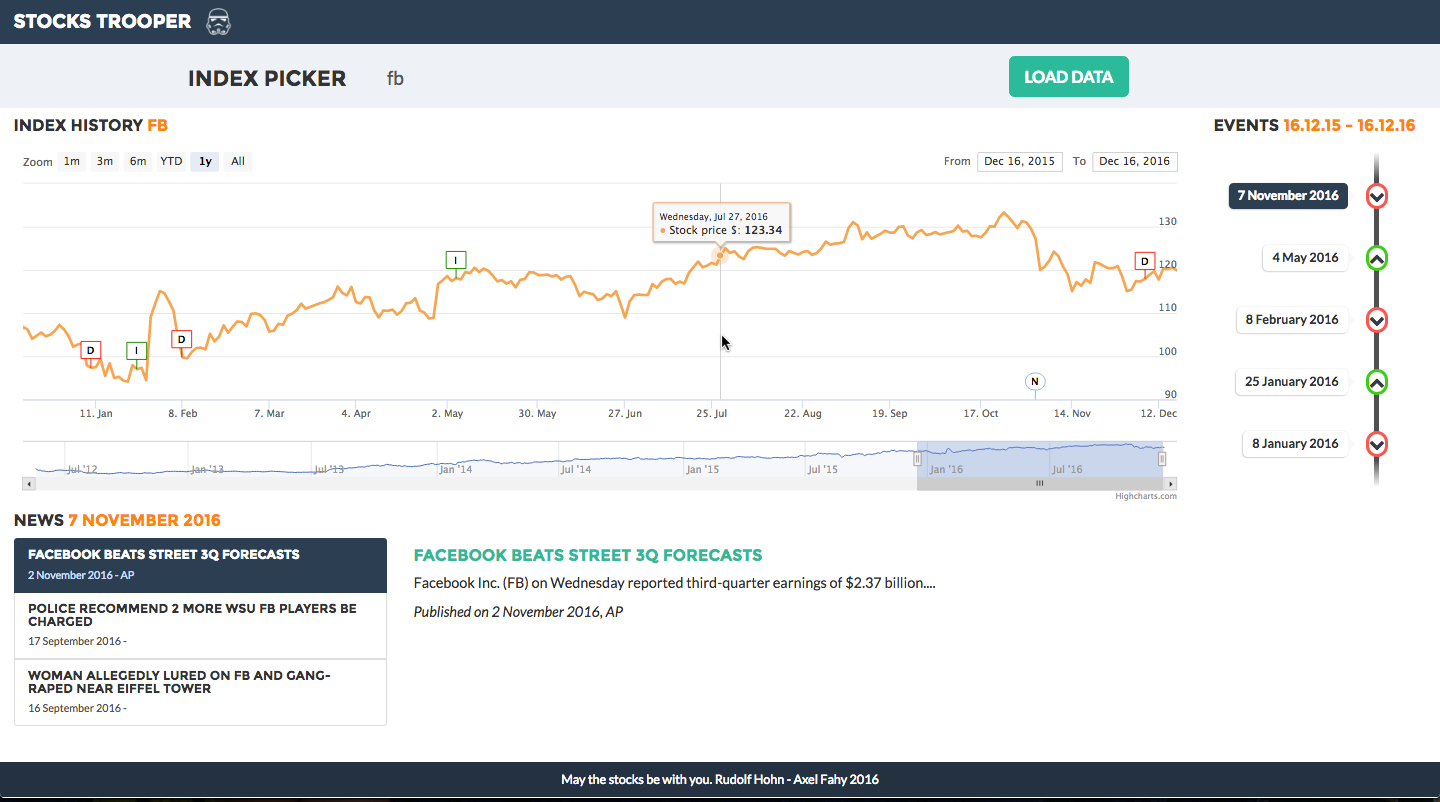
\includegraphics[max width=\textwidth]{Figures/st-full.png}
    \caption{Example of visualisation of the full application based on Facebook (FB) stock price.}
    \label{fig:full}
\end{figure}

%-------------------------------------------------------------------------------
%-------------------------------------------------------------------------------
\section{Easter egg}
This is a secret section. However, if you gently ask a Storm Trooper, he might reveal it.
